% TODO: This one is not finished yet!
\documentclass{article}

\usepackage{tikz}

\usetikzlibrary{decorations.pathreplacing}
\usetikzlibrary{fit}

\begin{document}

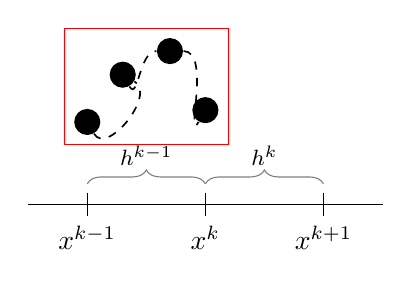
\begin{tikzpicture}[scale=1.5,dot/.style={fill=black,circle,minimum size=2pt}]

% x-axis
\draw[-] (-1.5,0) -- (1.5,0);
\draw (0, 0.1) -- (0, -0.1) node [below] {$x^k$};
\draw (-1, 0.1) -- (-1, -0.1) node [below] {$x^{k-1}$};
\draw (1, 0.1) -- (1, -0.1) node [below] {$x^{k+1}$};

% points
\node[dot] (a1) at (-1,0.7) {};
\node[dot] (b1) at (-0.7,1.1) {};
\node[dot] (c1) at (-0.3,1.3) {};
\node[dot] (d1) at (0,0.8) {};
\node[draw=red, fit=(a1) (b1) (c1) (d1)] {};

% line representing function
\draw [dashed, semithick]  
   (a1) to [out=-60,in=330] (b1)
   to [out=-60,in=180] (c1) 
   to [out=0,in=240] (d1);

\draw [gray,decorate,decoration={brace,amplitude=5pt},yshift=5pt]
   (0,0)  -- (1,0) 
   node [black,midway,above=3pt] {\footnotesize $h^k$};
\draw [gray,decorate,decoration={brace,amplitude=5pt},yshift=5pt]
   (-1,0)  -- (0,0) 
   node [black,midway,above=3pt] {\footnotesize $h^{k-1}$};

\end{tikzpicture}

\end{document}
